\documentclass[12pt,a4paper]{scrartcl}

\usepackage[utf8]{inputenc}
\usepackage[T1]{fontenc}
\usepackage[ngerman]{babel}
\usepackage{lmodern}
\usepackage{microtype}
\usepackage{geometry}
\usepackage{setspace}
\usepackage{graphicx}
\usepackage{float}
\usepackage{booktabs}
\usepackage{tabularx}
\usepackage{xcolor}
\usepackage{hyperref}
\usepackage{tikz}
\usepackage{pgfplots}
\usepackage{amsmath}

\pgfplotsset{compat=1.18}
\usetikzlibrary{arrows.meta,positioning,shapes.geometric}

\geometry{left=25mm,right=25mm,top=25mm,bottom=28mm}
\onehalfspacing
\setlength{\parindent}{0pt}
\setlength{\parskip}{0.65em}
\newcommand{\SI}[2]{#1\,#2}
\newcommand{\percent}{\%}

\definecolor{levelblue}{HTML}{1E88E5}
\definecolor{flowgreen}{HTML}{13A86B}
\definecolor{pressureorange}{HTML}{F2A51A}
\definecolor{pumpviolet}{HTML}{6C63FF}
\definecolor{valvered}{HTML}{D64E64}
\definecolor{gridgray}{HTML}{D9DEE7}

\hypersetup{
  colorlinks=true,
  linkcolor=black,
  urlcolor=levelblue,
  pdftitle={Dokumentation Wasserstandsregelung},
  pdfauthor={Hendrik Lappe}
}

\title{\textbf{Dokumentation der Wasserstandsregelung}\\[0.4em]
\large Regelungstechnik 2 -- Festo D:PA-KIT-MSR-MAN}
\author{Hendrik Lappe}
\date{\today}

\begin{document}

\begin{titlepage}
  \centering
  \vspace*{18mm}
  {\Huge\bfseries Wasserstandsregelung\\[0.25em]mit 3-Punkt-Regler\par}
  \vspace{8mm}
  {\Large Dokumentation zum Projekt in Regelungstechnik 2\par}
  \vspace{18mm}
  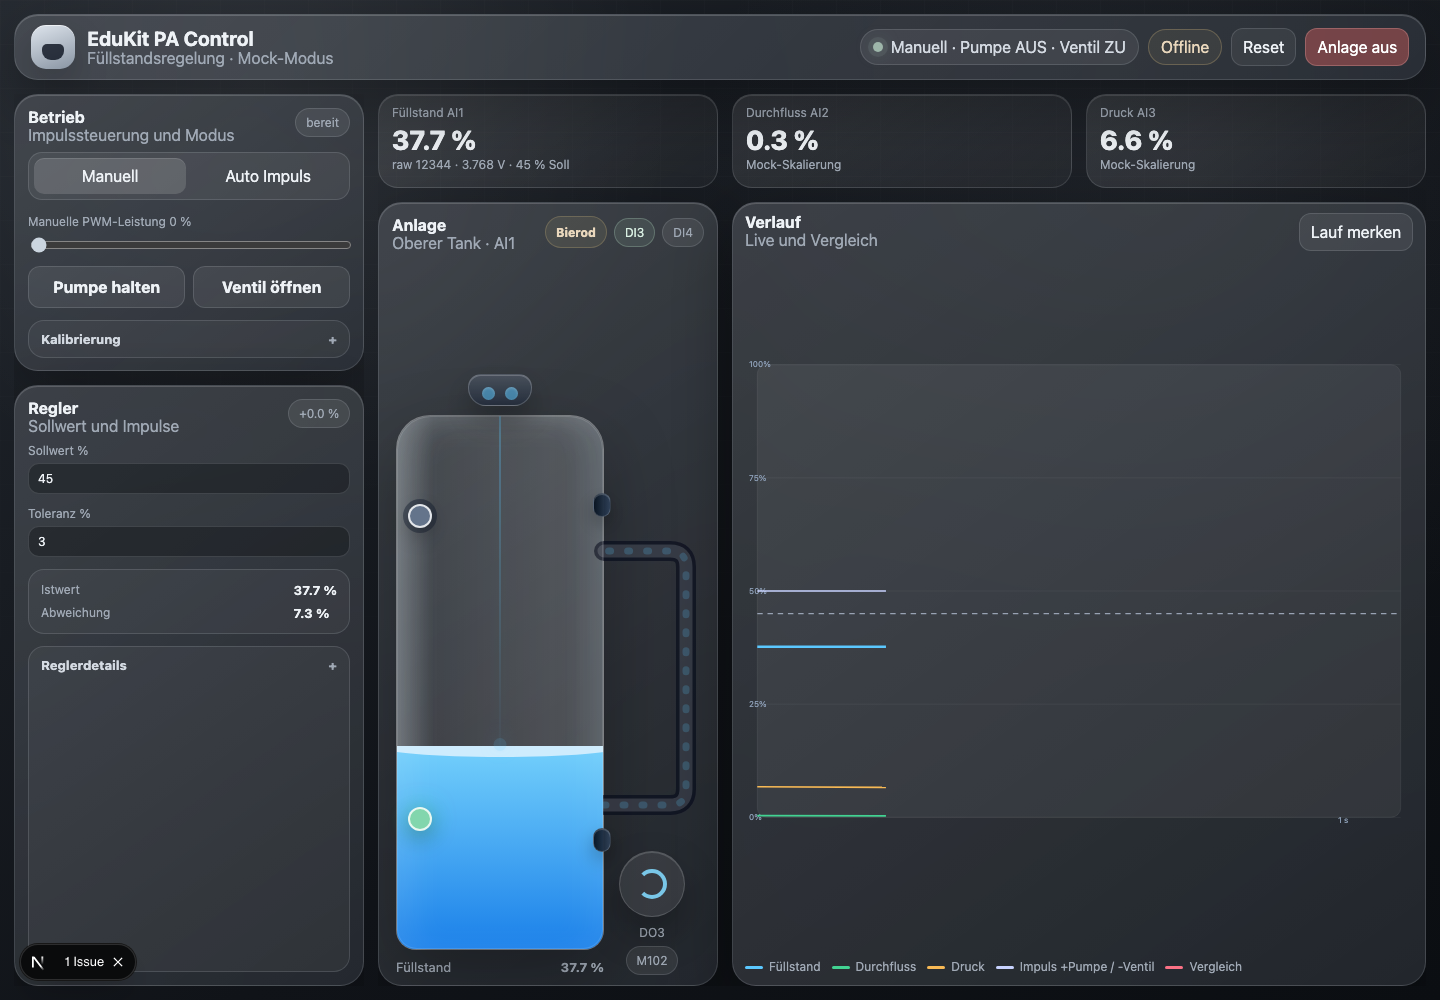
\includegraphics[width=0.86\textwidth]{figures/screenshots/dashboard-overview.png}
  \vfill
  \begin{tabular}{ll}
    System: & Festo D:PA-KIT-MSR-MAN mit EasyPort-Anbindung\\
    Software: & Python-API und Next.js-Dashboard\\
    Autor: & Hendrik Lappe\\
    Datum: & \today
  \end{tabular}
\end{titlepage}

\tableofcontents
\newpage

\section{Einleitung}

Ziel dieses Projekts ist der Aufbau einer automatisierten Wasserstandsregelung an einem didaktischen Prozessmodell. Der Füllstand eines oberen Tanks soll auf einen vorgegebenen Sollwert geregelt werden. Dazu werden Messwerte aus dem System erfasst, in einer Weboberfläche angezeigt und über eine digitale Pumpe sowie ein digitales Ablassventil beeinflusst.

Das Projekt verbindet damit mehrere typische Aufgaben der Regelungstechnik: die Erfassung einer Prozessgröße, die Skalierung eines Sensorsignals, die Analyse der Regelstrecke, die Auswahl einer passenden Reglerstruktur und die Bewertung des Systemverhaltens bei Sollwertänderungen und Störungen. Eine Besonderheit des Aufbaus ist, dass die Pumpe im verwendeten Aufbau nicht stetig stellbar ist, sondern nur digital ein- und ausgeschaltet werden kann. Dadurch ist ein klassischer PID-Regler für die Pumpe nicht sinnvoll umsetzbar. Stattdessen wird eine 3-Punkt-Regelung verwendet, bei der die drei Zustände \glqq Füllen\grqq, \glqq Halten\grqq{} und \glqq Ablassen\grqq{} gezielt eingesetzt werden.

Die Dokumentation beschreibt zunächst den Aufbau des Systems und die Zielsetzung. Anschließend wird erklärt, warum eine 3-Punkt-Regelung besser zum realen Aufbau passt als ein PID-Regler. Danach werden die Weboberfläche, die Kalibrierung und die verwendete Regelstrategie dargestellt. Abschließend werden Messungen zur Sprungantwort und zum Verhalten bei einer Störgröße vorbereitet und bewertet.

\section{Projektziel und Anforderungen}

Der obere Tank des Prozessmodells soll auf einen einstellbaren Füllstand geregelt werden. Der Benutzer gibt über die Weboberfläche einen Sollwert in Prozent vor. Die Regelung soll diesen Sollwert möglichst zuverlässig erreichen und danach stabil halten. Gleichzeitig soll das System verständlich, beobachtbar und im Laborbetrieb sicher bedienbar bleiben.

Die wichtigsten Anforderungen sind:

\begin{itemize}
  \item Anzeige von Füllstand, Durchfluss und Druck in einer Weboberfläche.
  \item Bedienung von Pumpe und Ventil im manuellen Modus.
  \item Automatischer Regelbetrieb mit Sollwertvorgabe.
  \item Kalibrierung des Füllstandssensors über Referenzpunkte.
  \item Sicheres Abschalten der Aktoren über die Oberfläche.
  \item Nachvollziehbare Darstellung des Regelverhaltens über Diagramme.
\end{itemize}

Das Projekt ist nicht nur als fertige Automatisierung zu verstehen, sondern auch als Lernsystem. Deshalb ist die Visualisierung des Prozesses ein wichtiger Bestandteil. Die Oberfläche zeigt nicht nur den aktuellen Wert, sondern auch den Verlauf und den aktuellen Zustand der Aktoren. Dadurch kann das Verhalten der Regelstrecke direkt mit der Regelentscheidung verglichen werden.

\section{Systemaufbau}

Der Aufbau besteht aus dem Festo D:PA-KIT-MSR-MAN, einer EasyPort-Schnittstelle, einem Python-Backend und einer Weboberfläche. Die EasyPort-Schnittstelle verbindet die reale Anlage mit dem Rechner. Über sie werden analoge Eingangswerte gelesen und digitale Ausgänge gesetzt.

\begin{table}[H]
  \centering
  \caption{Wichtige Komponenten des Projekts}
  \begin{tabularx}{\textwidth}{lX}
    \toprule
    Komponente & Aufgabe\\
    \midrule
    Oberer Tank & Regelgröße ist der Wasserstand im Tank.\\
    Füllstandssensor & Liefert den Rohwert des aktuellen Wasserstands.\\
    Pumpe & Fördert Wasser in Richtung oberer Tank. Im aktuellen Aufbau digital: an oder aus.\\
    Ablassventil M102 & Lässt Wasser aus dem Tank ab und dient als Stellglied zum feinen Absenken.\\
    Störventil & Zusätzliches Ventil, über das Wasser als Störgröße abgelassen werden kann.\\
    EasyPort & Erfasst Ein- und Ausgänge und stellt die Verbindung zur Software her.\\
    Python-API & Liest Messwerte, berechnet den Reglerzustand und schaltet Aktoren.\\
    Weboberfläche & Visualisiert den Prozess und erlaubt Bedienung, Kalibrierung und Sollwertvorgabe.\\
    \bottomrule
  \end{tabularx}
\end{table}

Die aktuelle Softwarestruktur ist in mehrere Dateien aufgeteilt. Der API-Server wird in Python umgesetzt. Er stellt den aktuellen Anlagenzustand über HTTP bereit und nimmt Bedienbefehle entgegen. Die Datei \texttt{control\_loop.py} enthält die Regelungslogik. In \texttt{edukit\_pa.py} wird der Zugriff auf die Anlage abstrahiert. Die Weboberfläche liegt im Ordner \texttt{frontend/} und ist als Next.js-Anwendung umgesetzt.

\section{Regelstrecke}

Die Regelstrecke beschreibt den Zusammenhang zwischen Stellgröße und Regelgröße. Im vorliegenden System ist die Regelgröße der Füllstand im oberen Tank. Die Stellgrößen sind Pumpe und Regelventil. Die Pumpe erhöht den Füllstand, das Ventil senkt ihn. Zusätzlich wirken Störgrößen, zum Beispiel ein extern geöffnetes Ablassventil oder Schwankungen durch Wellenbildung im Tank.

\begin{figure}[H]
  \centering
  \resizebox{\textwidth}{!}{%
  \begin{tikzpicture}[
    block/.style={draw, rounded corners, align=center, minimum width=28mm, minimum height=10mm},
    sum/.style={draw, circle, inner sep=1pt, minimum size=7mm},
    arrow/.style={-{Latex[length=2mm]}, thick}
  ]
    \node[block] (controller) {3-Punkt-\\Regler};
    \node[block, right=17mm of controller] (actuators) {Pumpe /\\Ventil};
    \node[block, right=17mm of actuators] (plant) {Tank, Rohrleitung,\\Totzeit};
    \node[block, right=17mm of plant] (sensor) {Füllstands-\\sensor};
    \node[sum, left=15mm of controller] (sum) {};
    \node[above=7mm of sum] (setpoint) {$w$: Sollwert};
    \node[below=13mm of plant] (disturbance) {$z$: Störabfluss};

    \draw[arrow] (setpoint) -- (sum);
    \draw[arrow] (sum) -- node[above] {$e=w-y$} (controller);
    \draw[arrow] (controller) -- node[above] {$u$} (actuators);
    \draw[arrow] (actuators) -- (plant);
    \draw[arrow] (disturbance) -- (plant);
    \draw[arrow] (plant) -- node[above] {$h$} (sensor);
    \draw[arrow] (sensor.east) -- ++(10mm,0) |- node[pos=0.25,right] {$y$} (sum.south);
  \end{tikzpicture}%
  }
  \caption{Vereinfachte Regelstrecke der Wasserstandsregelung}
\end{figure}

Die Strecke ist träge. Wenn die Pumpe eingeschaltet wird, ist der Effekt am oberen Tank nicht sofort vollständig sichtbar. Das Wasser muss erst durch Leitung und Aufbau transportiert werden. Dadurch entsteht eine Totzeit. Zusätzlich ist die Oberfläche des Wassers nicht ideal ruhig. Blasen, Wellen und Strömungen führen dazu, dass der gemessene Rohwert schwankt. Diese Eigenschaften machen eine vorsichtige Regelstrategie notwendig.

\section{Warum kein klassischer PID-Regler?}

Ein PID-Regler berechnet aus der Regelabweichung eine kontinuierliche Stellgröße. Diese Stellgröße kann beispielsweise \SI{0}{\percent} bis \SI{100}{\percent} betragen. Damit ein PID-Regler seine Vorteile ausspielen kann, muss das Stellglied diesen kontinuierlichen Wert auch umsetzen können. Bei einer drehzahlgeregelten Pumpe wäre das möglich: Der Regler könnte eine Pumpenleistung von \SI{23}{\percent}, \SI{48}{\percent} oder \SI{71}{\percent} vorgeben.

Im aktuellen Aufbau ist die Pumpe jedoch digital verschaltet. Sie kann nur \glqq aus\grqq{} oder \glqq an\grqq{} sein. Ein PID-Ausgang von beispielsweise \SI{37}{\percent} kann nicht direkt als \SI{37}{\percent} Pumpenleistung ausgegeben werden. Man könnte diesen Wert zwar über Pulsweitenmodulation annähern, das wäre aber bei der vorhandenen Totzeit und dem groben Förderverhalten schwer sauber einzustellen. Besonders der Integralanteil eines PID-Reglers kann bei solchen Ein-Aus-Stellgliedern problematisch werden, weil der Regler weiter aufintegriert, obwohl die Wirkung der Pumpe erst verspätet sichtbar wird.

Deshalb wird hier keine klassische PID-Regelung verwendet. Stattdessen passt eine 3-Punkt-Regelung besser zum realen System:

\begin{itemize}
  \item Ist der Füllstand zu niedrig, wird gefüllt.
  \item Liegt der Füllstand im Toleranzband, bleiben Pumpe und Ventil aus.
  \item Ist der Füllstand zu hoch, wird über das Ventil abgelassen.
\end{itemize}

Diese Logik entspricht direkt den vorhandenen Stellmöglichkeiten. Sie ist robuster gegenüber dem digitalen Verhalten der Aktoren und für den Laboraufbau besser nachvollziehbar.

\section{Aktuelle Regelstrategie}

Die aktuelle Regelung arbeitet nicht nach dem Prinzip, exakt bis zum Sollwert zu pumpen und dort sofort anzuhalten. Das wäre bei der vorhandenen Totzeit ungünstig. Wenn die Pumpe ausgeschaltet wird, ist noch Wasser unterwegs oder der gemessene Füllstand stabilisiert sich erst verzögert. Wird zu spät abgeschaltet, entsteht eine deutliche Überfüllung. Wird zu früh abgeschaltet, muss sofort wieder nachgepumpt werden.

Die verwendete Strategie nutzt deshalb bewusst die Eigenschaften des Systems: Bei zu niedrigem Füllstand wird mit der Pumpe grob gefüllt. Dabei wird ein gewisses Überfüllen oberhalb des Toleranzbands zugelassen. Anschließend wird nicht mit der Pumpe fein nachgeregelt, sondern über das Ablassventil in kleinen Takten abgesenkt. Dieses Vorgehen ist sinnvoll, weil das Ventil für kleine Korrekturen besser geeignet ist als die Pumpe. Die Pumpe hat eine Totzeit und bringt relativ viel Wasser ins System. Das Ventil kann dagegen kurze Korrekturen nach unten ausführen.

Die Regelung besteht aus mehreren Bereichen:

\begin{table}[H]
  \centering
  \caption{Bereiche der 3-Punkt-Regelung}
  \begin{tabularx}{\textwidth}{lX}
    \toprule
    Bereich & Verhalten\\
    \midrule
    Unterhalb des Sollwerts & Die Pumpe füllt den Tank.\\
    Im Toleranzband & Beide Aktoren bleiben aus. Der aktuelle Füllstand wird akzeptiert.\\
    Deutlich oberhalb des Sollwerts & Das Ventil bleibt geöffnet, bis der Füllstand näher an den Sollwert kommt.\\
    Nahe oberhalb des Sollwerts & Das Ventil öffnet nur in kurzen Takten.\\
    Sehr nahe am Sollwert & Das Ventil öffnet in sehr kurzen Feintakten.\\
    \bottomrule
  \end{tabularx}
\end{table}

Die Regelung ist damit eine hybride 3-Punkt-Regelung. Sie nutzt harte Schaltzustände, ergänzt diese aber durch kurze Ventilimpulse, um das System feiner in Richtung Sollwert zu bringen.

\section{Weboberfläche}

Die Weboberfläche dient als Bedien- und Beobachtungsebene. Sie zeigt den aktuellen Füllstand, Durchfluss und Druck sowie den Zustand von Pumpe und Ventil. Zusätzlich kann zwischen manuellem Betrieb und automatischer Impulsregelung umgeschaltet werden.

\begin{figure}[H]
  \centering
  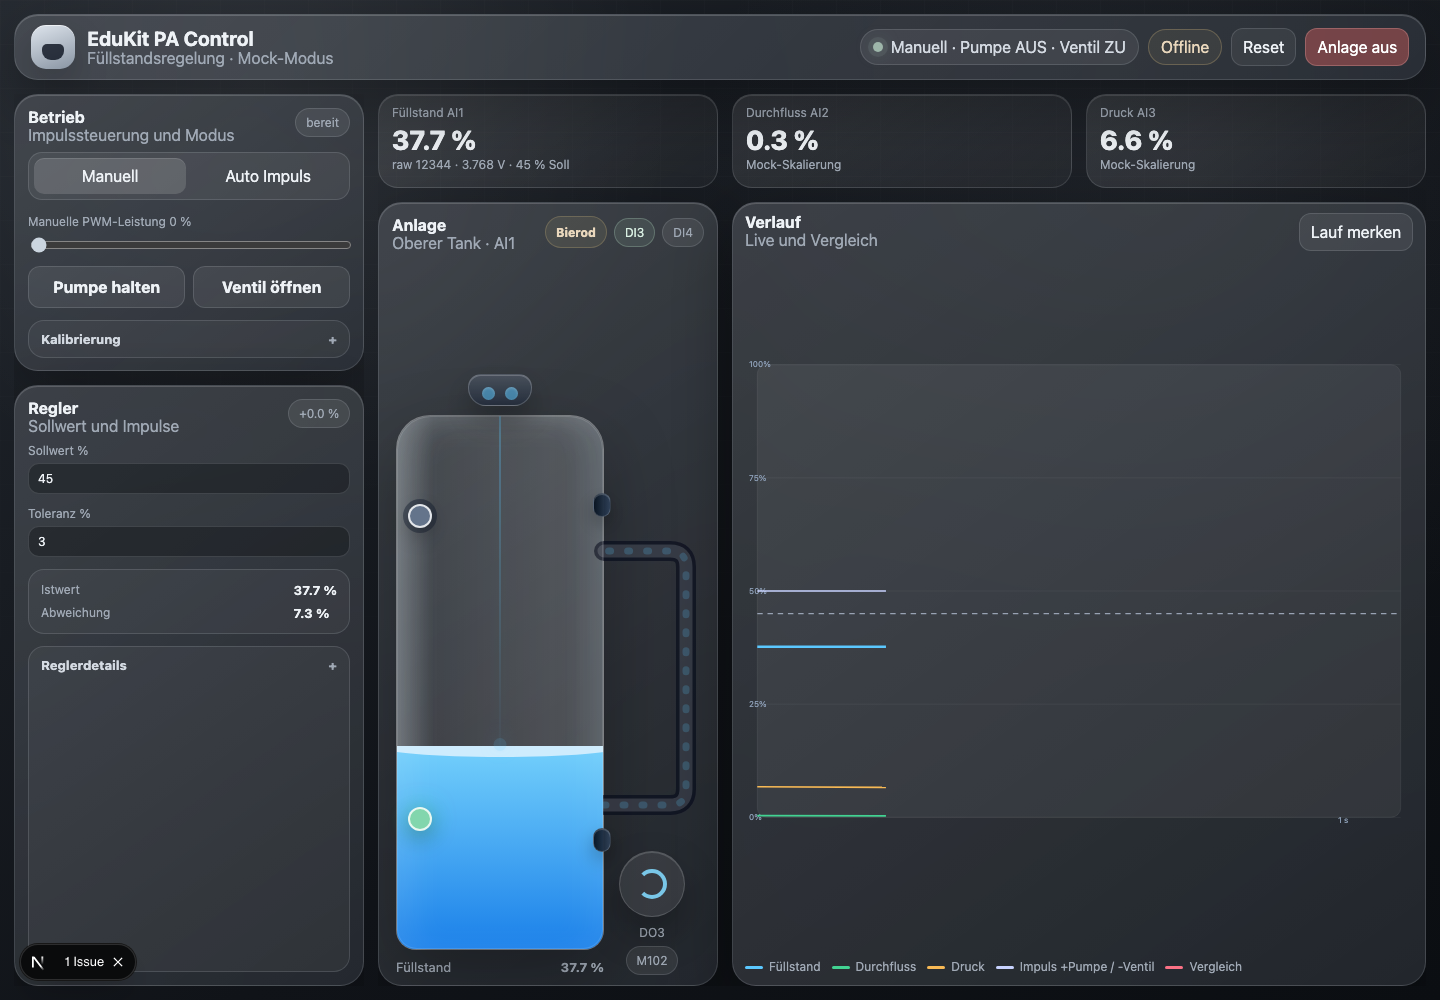
\includegraphics[width=\textwidth]{figures/screenshots/dashboard-overview.png}
  \caption{Weboberfläche des Dashboards}
\end{figure}

Links befindet sich der Bedienbereich. Dort kann der Modus gewählt werden. Im manuellen Modus können Pumpe und Ventil direkt bedient werden. Außerdem gibt es eine Kalibrierung für den Füllstand. Dabei wird ein unterer Referenzstand als \SI{0}{\percent} und ein oberer Referenzstand als \SI{100}{\percent} gespeichert. Aus diesen beiden Rohwerten berechnet die Software den angezeigten Prozentwert.

Im Reglerbereich werden Sollwert und Toleranz eingestellt. Die Toleranz legt fest, in welchem Bereich um den Sollwert herum nicht weiter geregelt wird. Dadurch wird verhindert, dass das System wegen kleiner Messschwankungen permanent zwischen Pumpe und Ventil wechselt.

Der mittlere Bereich visualisiert den Tank. Dadurch ist sofort sichtbar, ob sich die Anzeige plausibel zum realen Aufbau verhält. Rechts wird der Verlauf dargestellt. Diese Kurve ist besonders wichtig, um Regelvorgänge, Sprungantworten und Störungen auszuwerten.

\section{Kalibrierung des Füllstands}

Der Füllstandssensor liefert zunächst einen Rohwert. Dieser Rohwert muss auf einen Prozentwert umgerechnet werden. Die einfachste Kalibrierung verwendet zwei Punkte:

\begin{itemize}
  \item \textbf{0 \%}: Rohwert beim unteren Referenzfüllstand.
  \item \textbf{100 \%}: Rohwert beim oberen Referenzfüllstand.
\end{itemize}

Die lineare Skalierung lautet:

\[
  y = \frac{x - x_0}{x_{100} - x_0} \cdot 100
\]

Dabei ist \(x\) der aktuelle Rohwert, \(x_0\) der Rohwert bei \SI{0}{\percent} und \(x_{100}\) der Rohwert bei \SI{100}{\percent}. Der berechnete Wert \(y\) ist der Füllstand in Prozent.

In der Praxis ist wichtig, dass die Wasseroberfläche beim Speichern der Referenzwerte möglichst ruhig ist. Wellen und Blasen führen sonst dazu, dass der gespeicherte Rohwert nicht exakt zum sichtbaren Füllstand passt. Deshalb sollte vor dem Speichern kurz gewartet werden, bis sich die Oberfläche beruhigt hat.

\section{Sprungantwort der Strecke}

Zur Bewertung der Regelstrecke wird eine Sprungantwort aufgenommen. Dabei wird die Pumpe sprunghaft eingeschaltet und anschließend beobachtet, wie Füllstand, Durchfluss und Druck reagieren. Die Messung zeigt, wie träge das System ist und wie stark die Verzögerung zwischen Pumpenbefehl und sichtbarer Änderung im Tank ausfällt.

Die folgende Abbildung verwendet aktuell Platzhalterdaten aus \texttt{data/sprungantwort.csv}. Sobald die reale Messdatei vorliegt, muss nur diese CSV-Datei ersetzt werden. Die Spaltenstruktur ist:

\begin{center}
\texttt{t,pump,level,flow,pressure}
\end{center}

\begin{figure}[H]
  \centering
  \begin{tikzpicture}
    \begin{axis}[
      width=\textwidth,
      height=80mm,
      grid=both,
      grid style={gridgray},
      xlabel={Zeit in s},
      ylabel={Signal in \%},
      ymin=0,
      ymax=105,
      legend pos=south east,
      legend cell align=left
    ]
      \addplot[thick, levelblue] table[col sep=comma,x=t,y=level]{data/sprungantwort.csv};
      \addlegendentry{Füllstand}
      \addplot[thick, flowgreen] table[col sep=comma,x=t,y=flow]{data/sprungantwort.csv};
      \addlegendentry{Durchfluss}
      \addplot[thick, pressureorange] table[col sep=comma,x=t,y=pressure]{data/sprungantwort.csv};
      \addlegendentry{Druck}
      \addplot[thick, dashed, pumpviolet] table[col sep=comma,x=t,y=pump]{data/sprungantwort.csv};
      \addlegendentry{Pumpe}
    \end{axis}
  \end{tikzpicture}
  \caption{Sprungantwort der Strecke bei Pumpenaktivierung}
\end{figure}

Typisch ist, dass Durchfluss und Druck schneller reagieren als der Füllstand. Der Füllstand steigt verzögert, weil zunächst Wasser gefördert und transportiert werden muss. Genau diese Verzögerung begründet, warum die Regelung nicht aggressiv direkt auf den Sollwert pumpen sollte.

\section{Störgrößenversuch}

Neben der Sollwertfolge ist auch das Verhalten bei Störungen wichtig. Im Projekt kann über ein zusätzliches Ventil Wasser abgelassen werden, das nicht das eigentliche Regelventil ist. Dieses Ventil wirkt als Störgröße. Wird es geöffnet, sinkt der Füllstand, obwohl die Regelung diesen Abfluss nicht direkt als Stellbefehl verursacht.

Die Regelung muss darauf reagieren. Fällt der Füllstand unter das Toleranzband, wird die Pumpe aktiviert. Sobald der Füllstand wieder im gewünschten Bereich liegt oder oberhalb liegt, wird die Pumpe abgeschaltet und gegebenenfalls über das Regelventil nach unten korrigiert.

Die folgende Abbildung verwendet Platzhalterdaten aus \texttt{data/stoerung.csv}. Die spätere reale Messdatei sollte diese Spalten enthalten:

\begin{center}
\texttt{t,setpoint,level,pump,valve,disturbance}
\end{center}

\begin{figure}[H]
  \centering
  \begin{tikzpicture}
    \begin{axis}[
      width=\textwidth,
      height=82mm,
      grid=both,
      grid style={gridgray},
      xlabel={Zeit in s},
      ylabel={Signal in \%},
      ymin=0,
      ymax=105,
      legend pos=south east,
      legend cell align=left
    ]
      \addplot[thick, black] table[col sep=comma,x=t,y=setpoint]{data/stoerung.csv};
      \addlegendentry{Sollwert}
      \addplot[thick, levelblue] table[col sep=comma,x=t,y=level]{data/stoerung.csv};
      \addlegendentry{Füllstand}
      \addplot[thick, dashed, pumpviolet] table[col sep=comma,x=t,y=pump]{data/stoerung.csv};
      \addlegendentry{Pumpe}
      \addplot[thick, dashed, valvered] table[col sep=comma,x=t,y=valve]{data/stoerung.csv};
      \addlegendentry{Regelventil}
      \addplot[thick, dotted, pressureorange] table[col sep=comma,x=t,y=disturbance]{data/stoerung.csv};
      \addlegendentry{Störventil}
    \end{axis}
  \end{tikzpicture}
  \caption{Verhalten bei externer Störgröße durch zusätzliches Ablassventil}
\end{figure}

An diesem Versuch lässt sich bewerten, ob die Regelung nach einer Störung wieder in den Sollbereich zurückfindet. Besonders interessant sind dabei die maximale Abweichung, die Dauer bis zur Rückkehr in das Toleranzband und die Frage, ob die Regelung danach überschwingt.

\section{Bewertung des Regelverhaltens}

Die 3-Punkt-Regelung passt gut zum vorhandenen digitalen Aufbau. Sie ist verständlich und robust, solange die Schaltgrenzen und Taktzeiten passend gewählt sind. Ihre Grenzen liegen dort, wo sehr feines, kontinuierliches Nachregeln nötig wäre. Da die Pumpe nur ein- und ausgeschaltet wird, kann sie nicht beliebig kleine Korrekturen ausführen. Kleine Messschwankungen am Füllstand können außerdem dazu führen, dass die Regelung unruhig wirkt.

Der Ansatz, zuerst grob mit der Pumpe zu füllen und anschließend über das Ventil nach unten zu korrigieren, ist für diesen Aufbau nachvollziehbar. Er nutzt die Pumpe für das, was sie gut kann: Wasser schnell in das System bringen. Die Feinkorrektur erfolgt über das Ventil, weil kurze Ablassimpulse kontrollierter sind als sehr kurze Pumpenimpulse mit Totzeit.

Für die endgültige Bewertung sollten reale Messdaten verwendet werden. Wichtig sind insbesondere:

\begin{itemize}
  \item Überschwingen nach Pumpenaktivierung.
  \item Zeit bis zum Erreichen des Toleranzbands.
  \item Verhalten bei ruhigem und bei welligem Wasser.
  \item Reaktion auf externe Störabflüsse.
  \item Stabilität im eingeschwungenen Zustand.
\end{itemize}

\section{Fazit und Ausblick}

Im Projekt wurde eine Wasserstandsregelung für das Festo D:PA-KIT-MSR-MAN aufgebaut. Die Anlage wird über EasyPort mit einem Python-Backend verbunden und über eine Next.js-Weboberfläche bedient. Der Füllstand wird als Rohwert eingelesen, kalibriert und als Prozentwert dargestellt. Die Regelung arbeitet als 3-Punkt-Regelung mit den Zuständen Füllen, Halten und Ablassen.

Ein klassischer PID-Regler ist im aktuellen Aufbau nicht die passende Wahl, weil die Pumpe nicht kontinuierlich stellbar ist. Sie kann nur ein- oder ausgeschaltet werden. Die 3-Punkt-Regelung passt deshalb besser zu den real vorhandenen Aktoren. Durch die Totzeit zwischen Pumpenbefehl und sichtbarer Änderung im oberen Tank wird zusätzlich eine Strategie notwendig, die nicht versucht, exakt mit der Pumpe auf den Sollwert zu fahren. Stattdessen wird grob gefüllt und anschließend über das Ventil feiner nach unten korrigiert.

Für zukünftige Erweiterungen sind zwei Ansätze besonders interessant. Erstens könnte die Pumpe durch eine kontinuierlich regelbare Pumpe ersetzt oder mit einer belastbaren analogen Ansteuerung ausgestattet werden. Dann wäre eine echte PID-Regelung deutlich sinnvoller, weil der Regler eine kontinuierliche Stellgröße ausgeben könnte. Zweitens könnte die Füllstandsüberwachung durch eine Kamera ergänzt werden. Eine Kamera könnte helfen, Blasenbildung, Wellen und Reflexionen zu erkennen und aus der Messung herauszufiltern. Dadurch wäre eine robustere Bewertung des tatsächlichen Wasserstands möglich.

Die Dokumentation kann mit den realen CSV-Messdaten weiter vervollständigt werden. Besonders die Sprungantwort und der Störgrößenversuch sind entscheidend, um das Verhalten der Strecke quantitativ zu bewerten und die Regelstrategie nachvollziehbar zu begründen.

\end{document}
